\documentclass[12pt, a4paper]{article}
\usepackage[utf8]{inputenc}
\usepackage{amsmath}
\usepackage{amsthm}
\usepackage{amssymb}
\usepackage{graphicx}
\usepackage{parskip}
\usepackage{hyperref}
\usepackage{fancyhdr}
\usepackage{lastpage}
\usepackage[vlined,ruled]{algorithm2e}
\usepackage[acronym]{glossaries}
\usepackage{caption}
\usepackage{titlesec}
\usepackage{multirow}
\usepackage{tikz}
\usetikzlibrary{arrows}

\title{%
  Algorithmic Game Theory \\
  Homework 4
}
\author{%
  Juan Pablo Royo Sales\\
  \small{Universitat Politècnica de Catalunya}
}
\date\today

\pagestyle{fancy}
\fancyhf{}
\fancyhead[C]{}
\fancyhead[R]{Juan Pablo Royo Sales - UPC MIRI}
\fancyhead[L]{AGT - Homework 4}
\fancyfoot[L,C]{}
\fancyfoot[R]{Page \thepage{} of \pageref{LastPage}}
\setlength{\headheight}{15pt}
\renewcommand{\headrulewidth}{0.4pt}
\renewcommand{\footrulewidth}{0.4pt}

\renewcommand{\qedsymbol}{$\blacksquare$}

\begin{document}

\maketitle

\section{Problem 4}
\subsection{(a) Valuation Function}
Lets define a variable $x_i$ in which 
\[
x_{ij} = 
\begin{cases}
  1 \text{ if a copy of album } j \text{ is provided by player } i\\
  0 \text{ otherwise } 
\end{cases}
\]

Therefore, 

\begin{equation*}
  v(C) = \Biggr|\biggr\{j \mid \sum_{i \in C} x_{ij} \geq k \biggl\}\Biggl|\\
\end{equation*}

\subsection{(b) Is the game convex?}
\textbf{No, it is not convex because it is not super modular}.

Lets probe it by assuming that the game is super modular.
A game is \textbf{super modular} if $v(C \cup D) + v(C \cap D) \geq v(C) + v(D)$.

Lets take $2$ partitions $C$ and $D$ and lets assume that both partitions by itself has $ \geq k$ copies of some album $j$ but not each player by itself, therefore:

\begin{enumerate}
  \item $v(C) \geq 1 \land v(D) \geq 1$ because at least both partition can re-recording at least the album $j$.
  \item It can be seen by previous that $v(C \cup D) \geq 1$ because we are going to have at least 1 album recording of $j$ because one of the 2 partition group can provide at least $k$ copies and more if we join both.
  \item Lets suppose that the combination of both partition $C \cap D$ leads to a partition in which some players don't contribute copy of album $j$ because some of them contribute with players of partition $C$ and some other move to form coalition with players of partition $D$. In this case coalition $C \cap D$ is not reaching to at least $k$ of album $j$.
  \item By previous statement the only thing we can assure is that $v(C \cap D) \geq 0$ by non-negative condition on Cooperative Games.
  \item So we have that $v(C \cup D) + v(C \cap D) \geq 1$ and $v(C) + v(D) \geq 2$
\end{enumerate}

Therefore $v(C \cup D) + v(C \cap D) \ngeq v(C) + v(D)$

Then, \textbf{it is not convex.}

\subsection{(c) Shapley values}
Knowing that Shapley value is additive we can think on splitting up the game as the sum of several
Shapley values if they were different games, one for each album $j$.

Given that $S_{\pi}(i)$ is the list of predecessors, in this case \textbf{players} before $i$, that may or may not contribute with copy of album $j$.

We have 2 cases 
\begin{itemize}
  \item If $i$ does not have a copy of $j$, then $\Phi_i(\Gamma_j) = 0$
  \item If $i$ does, we need to count the number of possible permutation in which the other players have or not have $k-1$ copies of $j$
\end{itemize}

For that we know that if $v(S_{\pi}(i)) = 0$ and $i$ is added $v(S_{\pi}(i) \cup \{i\}) = 1$, \textit{if and only if} there is
$\sum_{a \in S_{\pi}(i)} x_{aj} = k - 1$. So we have that,

\begin{equation}
  \Phi_i(\Gamma_j) = \frac{|\{n | v(S_{\pi}(i)) = 0 \land v(S_{\pi}(i) \cup \{i\}) = 1\}|}{n!}
\end{equation}

So, we need to count the number of other players that has copies of $j$.

Lets define $b_j$ as the number of player that has copies of $j$.

Basically the permutation has the following form:

\begin{center}
  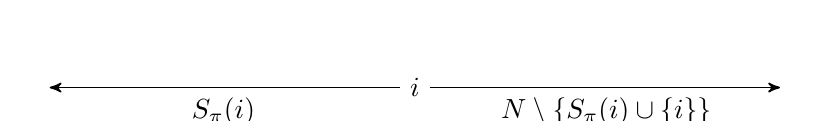
\begin{tikzpicture}[->,>=stealth',shorten >=1pt,auto,node distance=4.8cm,semithick]
    \node         (S)              {};
    \node         (i) [right of=S] {$i$};
    \node         (F) [right of=i] {};
    
    \path (i) edge node {$S_{\pi}(i)$} (S);
    \path (i) edge [below] node {$N \setminus \{S_{\pi}(i) \cup \{i\}\}$} (F);
  \end{tikzpicture}
\end{center}

In this picture, we can see that $S_{\pi}(i)$ has $k-1$ players with a copy of $j$ and the rest after $i$ does not.

Therefore we can argue that:

\[
  \begin{cases}
    | S_{\pi}(i) | \geq k-1 \\
    n - | S_{\pi}(i) | \geq b_j - k
  \end{cases}
\]

Plugin this equations together we have that 

\begin{equation}
  k-1 \leq | S_{\pi}(i) | \leq n - b_j - k
\end{equation}

Lets define this amount of players as $| S_{\pi}(i) | = \alpha$, so 

\begin{equation}
  k-1 \leq \alpha \leq n - b_j - k
\end{equation}

Graphically we can represent the number of players with:

\begin{center}
  \begin{tikzpicture}[->,>=stealth',shorten >=1pt,auto,node distance=4.8cm,semithick]
    \node         (S)              {};
    \node         (i) [right of=S] {$i$};
    \node         (F) [right of=i] {};
    
    \path (i) edge node {$\alpha$} (S);
    \path (i) edge [below] node {$n - \alpha - 1$} (F);
  \end{tikzpicture}
\end{center}

This means that $\alpha_i$ first players have $k-1$ copies of $j$ and the rest $n-\alpha-1$ does not.

So we need to count all possible combinations of players that has copies of $j$ and those who don't taking into consideration that $i$ has 1 copy.

\begin{equation}
  \binom{b_j - 1}{k-1}\binom{n-b_j}{\alpha - k - 1}
\end{equation}

So the total number of permutations when $v(S_{\pi}(i)) = 0 \land v(S_{\pi}(i) \cup \{i\}) = 1$, with $| S_{\pi}(i) | = \alpha$ is:

\begin{equation}
  \binom{b_j - 1}{k-1}\binom{n-b_j}{\alpha - k - 1} \alpha! (n - \alpha - 1)! 
\end{equation}

Therefore,

\begin{subequations}
  \begin{align} 
    \Phi_i(\Gamma) &= \frac{\sum_{\alpha = k -1}^{n-b_j-k} \binom{b_j - 1}{k-1}\binom{n-b_j}{\alpha - k - 1} \alpha! (n - \alpha - 1)!}{n!}\\
                   &= \frac{\binom{b_j - 1}{k-1}}{n!} \sum_{\alpha = k -1}^{n-b_j-k} \binom{n-b_j}{\alpha - k - 1} \alpha! (n - \alpha - 1)!
  \end{align}
\end{subequations}


Using additivity property of Shapley values if we telescope this to the sum of all games of different albums $j$

\begin{subequations}
  \begin{align}    
  \Phi_i(\Gamma) &= \Phi_i\bigr(\sum_{j=1}^M \Gamma_j\bigl)\\
                 &= \sum_{j=1}^M \Phi_i(\Gamma_j)\\
                 &= \sum_{j=1} \frac{\binom{b_j - 1}{k-1}}{n!} \sum_{\alpha = k -1}^{n-b_j-k} \binom{n-b_j}{\alpha - k - 1} \alpha! (n - \alpha - 1)!
  \end{align}
\end{subequations}

It cannot be calculated in \textit{Poly-time} because it has exponential number of permutation.

\end{document}

